% =====================================================================
%  (a) No Video Encoder -- trajectory-only baseline
%  Compile:  pdflatex arch_no_video.tex
% =====================================================================
\documentclass[tikz, border=10pt]{standalone}
\usepackage{amsmath,amssymb}
\usetikzlibrary{arrows.meta, positioning, fit, backgrounds, calc, shapes.geometric}

\tikzset{
  every node/.style={font=\small},
  io/.style   = {rectangle, rounded corners=3pt, draw=gray!60!black,   fill=gray!10,
                 inner sep=6pt, align=center, minimum height=1.0cm},
  kin/.style  = {rectangle, rounded corners=3pt, draw=blue!60!black,   fill=blue!15,
                 inner sep=6pt, align=center, minimum height=1.0cm},
  vid/.style  = {rectangle, rounded corners=3pt, draw=purple!60!black, fill=purple!15,
                 inner sep=6pt, align=center, minimum height=1.0cm},
  fuse/.style = {rectangle, rounded corners=3pt, draw=orange!80!black, fill=orange!20,
                 inner sep=6pt, align=center, minimum height=1.0cm},
  dec/.style  = {rectangle, rounded corners=3pt, draw=green!60!black,  fill=green!15,
                 inner sep=6pt, align=center, minimum height=1.0cm},
  vec/.style  = {rectangle, rounded corners=3pt, draw=blue!60!black,   fill=blue!8,
                 inner sep=4pt, align=center, font=\scriptsize, minimum height=0.7cm},
  arrow/.style = {-{Stealth[length=2.5mm,width=2mm]}, thick, rounded corners},
  title/.style = {font=\bfseries\small, align=center},
}

\begin{document}
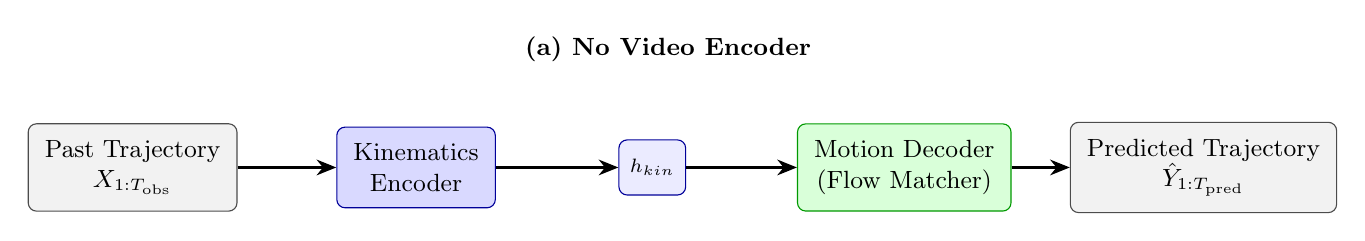
\begin{tikzpicture}
  \node[io]  (x)   at (0.0,0)  {Past Trajectory\\$X_{1:T_{\mathrm{obs}}}$};
  \node[kin] (enc) at (3.6,0)  {Kinematics\\Encoder};
  \node[vec] (h)   at (6.6,0)  {$h_{kin}$};
  \node[dec] (dec) at (9.8,0)  {Motion Decoder\\(Flow Matcher)};
  \node[io]  (y)   at (13.6,0) {Predicted Trajectory\\$\hat{Y}_{1:T_{\mathrm{pred}}}$};

  \draw[arrow] (x)   -- (enc);
  \draw[arrow] (enc) -- (h);
  \draw[arrow] (h)   -- (dec);
  \draw[arrow] (dec) -- (y);

  \node[title] at ($(x)!0.5!(y) + (0,1.5)$) {(a) No Video Encoder};
\end{tikzpicture}
\end{document}
